% Options for packages loaded elsewhere
% Options for packages loaded elsewhere
\PassOptionsToPackage{unicode}{hyperref}
\PassOptionsToPackage{hyphens}{url}
\PassOptionsToPackage{dvipsnames,svgnames,x11names}{xcolor}
%
\documentclass[
  spanish,
  11pt,
  a4paper,
  DIV=11,
  numbers=noendperiod]{scrartcl}
\usepackage{xcolor}
\usepackage[margin=2.5cm]{geometry}
\usepackage{amsmath,amssymb}
\setcounter{secnumdepth}{5}
\usepackage{iftex}
\ifPDFTeX
  \usepackage[T1]{fontenc}
  \usepackage[utf8]{inputenc}
  \usepackage{textcomp} % provide euro and other symbols
\else % if luatex or xetex
  \usepackage{unicode-math} % this also loads fontspec
  \defaultfontfeatures{Scale=MatchLowercase}
  \defaultfontfeatures[\rmfamily]{Ligatures=TeX,Scale=1}
\fi
\usepackage{lmodern}
\ifPDFTeX\else
  % xetex/luatex font selection
  \setmainfont[]{Times New Roman}
\fi
% Use upquote if available, for straight quotes in verbatim environments
\IfFileExists{upquote.sty}{\usepackage{upquote}}{}
\IfFileExists{microtype.sty}{% use microtype if available
  \usepackage[]{microtype}
  \UseMicrotypeSet[protrusion]{basicmath} % disable protrusion for tt fonts
}{}
\makeatletter
\@ifundefined{KOMAClassName}{% if non-KOMA class
  \IfFileExists{parskip.sty}{%
    \usepackage{parskip}
  }{% else
    \setlength{\parindent}{0pt}
    \setlength{\parskip}{6pt plus 2pt minus 1pt}}
}{% if KOMA class
  \KOMAoptions{parskip=half}}
\makeatother
% Make \paragraph and \subparagraph free-standing
\makeatletter
\ifx\paragraph\undefined\else
  \let\oldparagraph\paragraph
  \renewcommand{\paragraph}{
    \@ifstar
      \xxxParagraphStar
      \xxxParagraphNoStar
  }
  \newcommand{\xxxParagraphStar}[1]{\oldparagraph*{#1}\mbox{}}
  \newcommand{\xxxParagraphNoStar}[1]{\oldparagraph{#1}\mbox{}}
\fi
\ifx\subparagraph\undefined\else
  \let\oldsubparagraph\subparagraph
  \renewcommand{\subparagraph}{
    \@ifstar
      \xxxSubParagraphStar
      \xxxSubParagraphNoStar
  }
  \newcommand{\xxxSubParagraphStar}[1]{\oldsubparagraph*{#1}\mbox{}}
  \newcommand{\xxxSubParagraphNoStar}[1]{\oldsubparagraph{#1}\mbox{}}
\fi
\makeatother

\usepackage{color}
\usepackage{fancyvrb}
\newcommand{\VerbBar}{|}
\newcommand{\VERB}{\Verb[commandchars=\\\{\}]}
\DefineVerbatimEnvironment{Highlighting}{Verbatim}{commandchars=\\\{\}}
% Add ',fontsize=\small' for more characters per line
\usepackage{framed}
\definecolor{shadecolor}{RGB}{241,243,245}
\newenvironment{Shaded}{\begin{snugshade}}{\end{snugshade}}
\newcommand{\AlertTok}[1]{\textcolor[rgb]{0.68,0.00,0.00}{#1}}
\newcommand{\AnnotationTok}[1]{\textcolor[rgb]{0.37,0.37,0.37}{#1}}
\newcommand{\AttributeTok}[1]{\textcolor[rgb]{0.40,0.45,0.13}{#1}}
\newcommand{\BaseNTok}[1]{\textcolor[rgb]{0.68,0.00,0.00}{#1}}
\newcommand{\BuiltInTok}[1]{\textcolor[rgb]{0.00,0.23,0.31}{#1}}
\newcommand{\CharTok}[1]{\textcolor[rgb]{0.13,0.47,0.30}{#1}}
\newcommand{\CommentTok}[1]{\textcolor[rgb]{0.37,0.37,0.37}{#1}}
\newcommand{\CommentVarTok}[1]{\textcolor[rgb]{0.37,0.37,0.37}{\textit{#1}}}
\newcommand{\ConstantTok}[1]{\textcolor[rgb]{0.56,0.35,0.01}{#1}}
\newcommand{\ControlFlowTok}[1]{\textcolor[rgb]{0.00,0.23,0.31}{\textbf{#1}}}
\newcommand{\DataTypeTok}[1]{\textcolor[rgb]{0.68,0.00,0.00}{#1}}
\newcommand{\DecValTok}[1]{\textcolor[rgb]{0.68,0.00,0.00}{#1}}
\newcommand{\DocumentationTok}[1]{\textcolor[rgb]{0.37,0.37,0.37}{\textit{#1}}}
\newcommand{\ErrorTok}[1]{\textcolor[rgb]{0.68,0.00,0.00}{#1}}
\newcommand{\ExtensionTok}[1]{\textcolor[rgb]{0.00,0.23,0.31}{#1}}
\newcommand{\FloatTok}[1]{\textcolor[rgb]{0.68,0.00,0.00}{#1}}
\newcommand{\FunctionTok}[1]{\textcolor[rgb]{0.28,0.35,0.67}{#1}}
\newcommand{\ImportTok}[1]{\textcolor[rgb]{0.00,0.46,0.62}{#1}}
\newcommand{\InformationTok}[1]{\textcolor[rgb]{0.37,0.37,0.37}{#1}}
\newcommand{\KeywordTok}[1]{\textcolor[rgb]{0.00,0.23,0.31}{\textbf{#1}}}
\newcommand{\NormalTok}[1]{\textcolor[rgb]{0.00,0.23,0.31}{#1}}
\newcommand{\OperatorTok}[1]{\textcolor[rgb]{0.37,0.37,0.37}{#1}}
\newcommand{\OtherTok}[1]{\textcolor[rgb]{0.00,0.23,0.31}{#1}}
\newcommand{\PreprocessorTok}[1]{\textcolor[rgb]{0.68,0.00,0.00}{#1}}
\newcommand{\RegionMarkerTok}[1]{\textcolor[rgb]{0.00,0.23,0.31}{#1}}
\newcommand{\SpecialCharTok}[1]{\textcolor[rgb]{0.37,0.37,0.37}{#1}}
\newcommand{\SpecialStringTok}[1]{\textcolor[rgb]{0.13,0.47,0.30}{#1}}
\newcommand{\StringTok}[1]{\textcolor[rgb]{0.13,0.47,0.30}{#1}}
\newcommand{\VariableTok}[1]{\textcolor[rgb]{0.07,0.07,0.07}{#1}}
\newcommand{\VerbatimStringTok}[1]{\textcolor[rgb]{0.13,0.47,0.30}{#1}}
\newcommand{\WarningTok}[1]{\textcolor[rgb]{0.37,0.37,0.37}{\textit{#1}}}

\usepackage{longtable,booktabs,array}
\usepackage{calc} % for calculating minipage widths
% Correct order of tables after \paragraph or \subparagraph
\usepackage{etoolbox}
\makeatletter
\patchcmd\longtable{\par}{\if@noskipsec\mbox{}\fi\par}{}{}
\makeatother
% Allow footnotes in longtable head/foot
\IfFileExists{footnotehyper.sty}{\usepackage{footnotehyper}}{\usepackage{footnote}}
\makesavenoteenv{longtable}
\usepackage{graphicx}
\makeatletter
\newsavebox\pandoc@box
\newcommand*\pandocbounded[1]{% scales image to fit in text height/width
  \sbox\pandoc@box{#1}%
  \Gscale@div\@tempa{\textheight}{\dimexpr\ht\pandoc@box+\dp\pandoc@box\relax}%
  \Gscale@div\@tempb{\linewidth}{\wd\pandoc@box}%
  \ifdim\@tempb\p@<\@tempa\p@\let\@tempa\@tempb\fi% select the smaller of both
  \ifdim\@tempa\p@<\p@\scalebox{\@tempa}{\usebox\pandoc@box}%
  \else\usebox{\pandoc@box}%
  \fi%
}
% Set default figure placement to htbp
\def\fps@figure{htbp}
\makeatother



\ifLuaTeX
\usepackage[bidi=basic]{babel}
\else
\usepackage[bidi=default]{babel}
\fi
\ifPDFTeX
\else
\babelfont{rm}[]{Times New Roman}
\fi
% get rid of language-specific shorthands (see #6817):
\let\LanguageShortHands\languageshorthands
\def\languageshorthands#1{}


\setlength{\emergencystretch}{3em} % prevent overfull lines

\providecommand{\tightlist}{%
  \setlength{\itemsep}{0pt}\setlength{\parskip}{0pt}}



 


\usepackage[hidelinks]{hyperref}
\KOMAoption{captions}{tableheading}
\makeatletter
\@ifpackageloaded{caption}{}{\usepackage{caption}}
\AtBeginDocument{%
\ifdefined\contentsname
  \renewcommand*\contentsname{Tabla de contenidos}
\else
  \newcommand\contentsname{Tabla de contenidos}
\fi
\ifdefined\listfigurename
  \renewcommand*\listfigurename{Listado de Figuras}
\else
  \newcommand\listfigurename{Listado de Figuras}
\fi
\ifdefined\listtablename
  \renewcommand*\listtablename{Listado de Tablas}
\else
  \newcommand\listtablename{Listado de Tablas}
\fi
\ifdefined\figurename
  \renewcommand*\figurename{Figura}
\else
  \newcommand\figurename{Figura}
\fi
\ifdefined\tablename
  \renewcommand*\tablename{Tabla}
\else
  \newcommand\tablename{Tabla}
\fi
}
\@ifpackageloaded{float}{}{\usepackage{float}}
\floatstyle{ruled}
\@ifundefined{c@chapter}{\newfloat{codelisting}{h}{lop}}{\newfloat{codelisting}{h}{lop}[chapter]}
\floatname{codelisting}{Listado}
\newcommand*\listoflistings{\listof{codelisting}{Listado de Listados}}
\makeatother
\makeatletter
\makeatother
\makeatletter
\@ifpackageloaded{caption}{}{\usepackage{caption}}
\@ifpackageloaded{subcaption}{}{\usepackage{subcaption}}
\makeatother
\usepackage{bookmark}
\IfFileExists{xurl.sty}{\usepackage{xurl}}{} % add URL line breaks if available
\urlstyle{same}
\hypersetup{
  pdftitle={CCA-RDA},
  pdfauthor={Santos G},
  pdflang={es},
  colorlinks=true,
  linkcolor={blue},
  filecolor={Maroon},
  citecolor={Blue},
  urlcolor={Blue},
  pdfcreator={LaTeX via pandoc}}


\title{CCA-RDA}
\author{Santos G}
\date{}
\begin{document}
\maketitle

\renewcommand*\contentsname{Tabla de contenidos}
{
\hypersetup{linkcolor=}
\setcounter{tocdepth}{2}
\tableofcontents
}

\section{Contexto de proyecto
(CCA-RDA)}\label{contexto-de-proyecto-cca-rda}

El presente análisis busca comprender cómo las variaciones en la
composición de especies vegetales entre sitios se relacionan con
gradientes ambientales edáficos y químicos. Para ello, se aplican
métodos de ordenación multivariada que permiten resumir la compleja
estructura de los datos y explorar las asociaciones entre comunidades
biológicas y variables ambientales. El enfoque CCA/RDA amplía la
interpretación al incorporar explícitamente la relación entre las
especies y los gradientes ambientales medidos. Estas técnicas permiten
identificar qué variables explican la mayor parte de la variación en la
composición florística y visualizar los principales ejes ecológicos que
estructuran la comunidad.

\section{Carga de librerías y
dataset}\label{carga-de-libreruxedas-y-dataset}

\begin{Shaded}
\begin{Highlighting}[numbers=left,,]
\CommentTok{\# Librerías principales}
\FunctionTok{library}\NormalTok{(tidyverse)   }\CommentTok{\# manipulación y ggplot2}
\FunctionTok{library}\NormalTok{(vegan)       }\CommentTok{\# rda(), cca(), anova.cca(), vif.cca(), decostand()}
\FunctionTok{library}\NormalTok{(knitr)       }\CommentTok{\# kable()}
\FunctionTok{library}\NormalTok{(ggrepel)     }\CommentTok{\# etiquetas en ggplot}
\FunctionTok{library}\NormalTok{(broom)       }\CommentTok{\# tidy() si lo necesitas}

\CommentTok{\# Datos de ejemplo}
\FunctionTok{data}\NormalTok{(varespec)}
\FunctionTok{data}\NormalTok{(varechem)}
\end{Highlighting}
\end{Shaded}

\section{Preparación de datos y
transformaciones}\label{preparaciuxf3n-de-datos-y-transformaciones}

\begin{Shaded}
\begin{Highlighting}[numbers=left,,]
\CommentTok{\#  Comprobar dimensiones de las matrices}

\NormalTok{dims }\OtherTok{\textless{}{-}} \FunctionTok{tibble}\NormalTok{(}
\AttributeTok{objeto =} \FunctionTok{c}\NormalTok{(}\StringTok{"varespec (especies)"}\NormalTok{, }\StringTok{"varechem (ambientales)"}\NormalTok{),}
\AttributeTok{filas =} \FunctionTok{c}\NormalTok{(}\FunctionTok{nrow}\NormalTok{(varespec), }\FunctionTok{nrow}\NormalTok{(varechem)),}
\AttributeTok{columnas =} \FunctionTok{c}\NormalTok{(}\FunctionTok{ncol}\NormalTok{(varespec), }\FunctionTok{ncol}\NormalTok{(varechem))}
\NormalTok{)}
\NormalTok{knitr}\SpecialCharTok{::}\FunctionTok{kable}\NormalTok{(dims)}
\end{Highlighting}
\end{Shaded}

\begin{longtable}[]{@{}lrr@{}}

\caption{\label{tbl-cca-dimensiones}Dimensiones de los conjuntos de
datos biológicos (varespec) y ambientales (varechem)}

\tabularnewline

\toprule\noalign{}
objeto & filas & columnas \\
\midrule\noalign{}
\endhead
\bottomrule\noalign{}
\endlastfoot
varespec (especies) & 24 & 44 \\
varechem (ambientales) & 24 & 14 \\

\end{longtable}

\begin{Shaded}
\begin{Highlighting}[numbers=left,,]
\CommentTok{\#  Revisar rareza (proporción de ceros)}

\NormalTok{zero\_prop }\OtherTok{\textless{}{-}} \FunctionTok{tibble}\NormalTok{(}
\AttributeTok{variable =} \FunctionTok{colnames}\NormalTok{(varespec),}
\AttributeTok{prop\_zero =} \FunctionTok{colSums}\NormalTok{(varespec }\SpecialCharTok{==} \DecValTok{0}\NormalTok{) }\SpecialCharTok{/} \FunctionTok{nrow}\NormalTok{(varespec)}
\NormalTok{)}

\NormalTok{zero\_prop }\SpecialCharTok{\%\textgreater{}\%}
\FunctionTok{arrange}\NormalTok{(}\FunctionTok{desc}\NormalTok{(prop\_zero)) }\SpecialCharTok{\%\textgreater{}\%}
\FunctionTok{head}\NormalTok{(}\DecValTok{6}\NormalTok{) }\SpecialCharTok{\%\textgreater{}\%}
\NormalTok{knitr}\SpecialCharTok{::}\FunctionTok{kable}\NormalTok{(}\AttributeTok{digits =} \DecValTok{3}\NormalTok{)}
\end{Highlighting}
\end{Shaded}

\begin{longtable}[]{@{}lr@{}}

\caption{\label{tbl-cca-ceros}Proporción de ceros en las primeras seis
especies de la matriz de abundancias}

\tabularnewline

\toprule\noalign{}
variable & prop\_zero \\
\midrule\noalign{}
\endhead
\bottomrule\noalign{}
\endlastfoot
Betupube & 0.875 \\
Cladamau & 0.875 \\
Cladcerv & 0.875 \\
Hylosple & 0.833 \\
Icmaeric & 0.833 \\
Cladphyl & 0.833 \\

\end{longtable}

\begin{Shaded}
\begin{Highlighting}[numbers=left,,]
\CommentTok{\# Transformaciones para análisis}

\NormalTok{varespec\_hel }\OtherTok{\textless{}{-}} \FunctionTok{decostand}\NormalTok{(varespec, }\AttributeTok{method =} \StringTok{"hellinger"}\NormalTok{)  }\CommentTok{\# para RDA}
\NormalTok{varespec\_log  }\OtherTok{\textless{}{-}} \FunctionTok{decostand}\NormalTok{(varespec, }\AttributeTok{method =} \StringTok{"log"}\NormalTok{, }\AttributeTok{na.rm =} \ConstantTok{TRUE}\NormalTok{)  }\CommentTok{\# para CCA}

\CommentTok{\#  Escalar variables ambientales}

\NormalTok{varechem\_scaled }\OtherTok{\textless{}{-}} \FunctionTok{scale}\NormalTok{(varechem)}
\end{Highlighting}
\end{Shaded}

Antes de realizar los análisis de ordenación canónica (CCA y RDA), se
verificó la estructura de los datos biológicos (\texttt{varespec}) y
ambientales (\texttt{varechem}), estos muestran que ambos conjuntos de
datos poseen el mismo número de filas (sitios de muestreo), garantizando
la correspondencia entre las matrices de especies y variables
ambientales (ver Tabla~\ref{tbl-cca-dimensiones}).

Posteriormente, se evaluó la proporción de ceros en la matriz de
abundancias de especies (ver Tabla~\ref{tbl-cca-ceros}). Una alta
proporción de ceros es común en datos ecológicos, ya que muchas especies
presentan distribuciones restringidas o baja frecuencia en los sitios.
Sin embargo, valores excesivos pueden generar sesgos en los métodos
lineales, lo que justifica la aplicación de transformaciones previas.

En este caso, se aplicaron dos transformaciones complementarias:

\begin{itemize}
\item
  \textbf{Transformación de Hellinger}
  (\texttt{decostand(...,\ method\ =\ "hellinger")}), adecuada para
  análisis de redundancia (RDA), ya que suaviza la influencia de
  especies muy abundantes y permite el uso de métodos basados en
  distancias euclidianas.
\item
  \textbf{Transformación logarítmica}
  (\texttt{decostand(...,\ method\ =\ "log")}), recomendada para la CCA,
  que asume relaciones unimodales entre especies y gradientes
  ambientales.
\end{itemize}

Finalmente, las variables ambientales se escalaron (\texttt{scale()}),
asegurando que todas contribuyan de manera comparable a los análisis,
independientemente de sus unidades originales.

\section{Colinealidad en variables ambientales
(VIF)}\label{colinealidad-en-variables-ambientales-vif}

\begin{Shaded}
\begin{Highlighting}[numbers=left,,]
\CommentTok{\# Modelo RDA preliminar para evaluar VIF}
\NormalTok{rda\_prelim }\OtherTok{\textless{}{-}} \FunctionTok{rda}\NormalTok{(varespec\_hel }\SpecialCharTok{\textasciitilde{}}\NormalTok{ ., }\AttributeTok{data =} \FunctionTok{as.data.frame}\NormalTok{(varechem\_scaled))}
\NormalTok{vif\_vals }\OtherTok{\textless{}{-}} \FunctionTok{vif.cca}\NormalTok{(rda\_prelim)  }\CommentTok{\# VIF por variable en vegan}
\NormalTok{vif\_tbl }\OtherTok{\textless{}{-}} \FunctionTok{tibble}\NormalTok{(}\AttributeTok{variable =} \FunctionTok{names}\NormalTok{(vif\_vals), }\AttributeTok{VIF =} \FunctionTok{round}\NormalTok{(vif\_vals, }\DecValTok{3}\NormalTok{))}
\NormalTok{knitr}\SpecialCharTok{::}\FunctionTok{kable}\NormalTok{(vif\_tbl)}
\end{Highlighting}
\end{Shaded}

\begin{longtable}[]{@{}lr@{}}

\caption{\label{tbl-cca-rda-vif}VIF (inflación de la varianza) para
variables ambientales (modelo RDA preliminar)}

\tabularnewline

\toprule\noalign{}
variable & VIF \\
\midrule\noalign{}
\endhead
\bottomrule\noalign{}
\endlastfoot
N & 1.884 \\
P & 6.185 \\
K & 11.747 \\
Ca & 9.826 \\
Mg & 9.595 \\
S & 18.461 \\
Al & 20.332 \\
Fe & 8.849 \\
Mn & 5.168 \\
Zn & 7.755 \\
Mo & 4.575 \\
Baresoil & 2.213 \\
Humdepth & 5.639 \\
pH & 6.910 \\

\end{longtable}

Se presentan los valores del Factor de Inflación de la Varianza (VIF)
para cada variable ambiental incluida en el modelo RDA preliminar (ver
Tabla~\ref{tbl-cca-rda-vif}). El VIF mide cuánto se incrementa la
varianza de un coeficiente debido a la colinealidad con las demás
variables. En este caso, las variables S (18.46) y Al (20.33) presentan
colinealidad excesiva y deberían eliminarse o combinarse con otras
relacionadas antes de ajustar el modelo final. Además, K (11.75) y Ca
(9.83) están en el límite superior y podrían retenerse con precaución o
someterse a una selección posterior basada en significancia ecológica o
estadística.

\section{RDA: ajuste, tests y resumen}\label{rda-ajuste-tests-y-resumen}

\begin{Shaded}
\begin{Highlighting}[numbers=left,,]
\CommentTok{\#  Calcular VIF para identificar colinealidad}

\NormalTok{vif\_vals }\OtherTok{\textless{}{-}} \FunctionTok{vif.cca}\NormalTok{(}\FunctionTok{rda}\NormalTok{(varespec\_hel }\SpecialCharTok{\textasciitilde{}}\NormalTok{ .,}
\AttributeTok{data =} \FunctionTok{as.data.frame}\NormalTok{(varechem\_scaled)))}
\NormalTok{vif\_tbl }\OtherTok{\textless{}{-}} \FunctionTok{tibble}\NormalTok{(}\AttributeTok{variable =} \FunctionTok{names}\NormalTok{(vif\_vals), }\AttributeTok{VIF =}\NormalTok{ vif\_vals)}

\CommentTok{\# Seleccionar variables con VIF \textless{}= 10}

\NormalTok{vars\_select }\OtherTok{\textless{}{-}}\NormalTok{ vif\_tbl }\SpecialCharTok{\%\textgreater{}\%}
\FunctionTok{filter}\NormalTok{(VIF }\SpecialCharTok{\textless{}=} \DecValTok{10}\NormalTok{) }\SpecialCharTok{\%\textgreater{}\%}
\FunctionTok{pull}\NormalTok{(variable)}

\CommentTok{\# Ajustar modelo RDA con variables depuradas}

\NormalTok{form }\OtherTok{\textless{}{-}} \FunctionTok{as.formula}\NormalTok{(}\FunctionTok{paste}\NormalTok{(}\StringTok{"varespec\_hel \textasciitilde{}"}\NormalTok{, }\FunctionTok{paste}\NormalTok{(vars\_select,}
\AttributeTok{collapse =} \StringTok{" + "}\NormalTok{)))}
\NormalTok{rda\_mod2 }\OtherTok{\textless{}{-}} \FunctionTok{rda}\NormalTok{(form, }\AttributeTok{data =} \FunctionTok{as.data.frame}\NormalTok{(varechem\_scaled))}

\CommentTok{\# Evaluaciones estadísticas}

\NormalTok{anova\_rda\_global }\OtherTok{\textless{}{-}} \FunctionTok{anova.cca}\NormalTok{(rda\_mod2, }\AttributeTok{permutations =} \DecValTok{999}\NormalTok{)}
\NormalTok{anova\_rda\_axes   }\OtherTok{\textless{}{-}} \FunctionTok{anova.cca}\NormalTok{(rda\_mod2, }\AttributeTok{by =} \StringTok{"axis"}\NormalTok{, }\AttributeTok{permutations =} \DecValTok{999}\NormalTok{)}
\NormalTok{anova\_rda\_terms  }\OtherTok{\textless{}{-}} \FunctionTok{anova.cca}\NormalTok{(rda\_mod2, }\AttributeTok{by =} \StringTok{"terms"}\NormalTok{, }\AttributeTok{permutations =} \DecValTok{999}\NormalTok{)}

\CommentTok{\# Tabla de resultados}

\NormalTok{knitr}\SpecialCharTok{::}\FunctionTok{kable}\NormalTok{(broom}\SpecialCharTok{::}\FunctionTok{tidy}\NormalTok{(anova\_rda\_global))}
\end{Highlighting}
\end{Shaded}

\begin{longtable}[]{@{}lrrrr@{}}

\caption{\label{tbl-anova-global-rda}ANOVA global RDA depurado
(permutaciones)}

\tabularnewline

\toprule\noalign{}
term & df & Variance & statistic & p.value \\
\midrule\noalign{}
\endhead
\bottomrule\noalign{}
\endlastfoot
Model & 11 & 0.2139955 & 1.54933 & 0.032 \\
Residual & 12 & 0.1506778 & NA & NA \\

\end{longtable}

El modelo RDA depurado resultó estadísticamente significativo (F = 1.55,
p = 0.032), lo que indica que las variables ambientales seleccionadas
explican una proporción relevante de la variación en la composición de
especies (ver Tabla~\ref{tbl-anova-global-rda}).

\begin{Shaded}
\begin{Highlighting}[numbers=left,,]
\CommentTok{\# Tabla ANOVA por ejes}

\NormalTok{knitr}\SpecialCharTok{::}\FunctionTok{kable}\NormalTok{(broom}\SpecialCharTok{::}\FunctionTok{tidy}\NormalTok{(anova\_rda\_axes))}
\end{Highlighting}
\end{Shaded}

\begin{longtable}[]{@{}lrrrr@{}}

\caption{\label{tbl-anova-ejes-rda}ANOVA por ejes RDA depurado}

\tabularnewline

\toprule\noalign{}
term & df & Variance & statistic & p.value \\
\midrule\noalign{}
\endhead
\bottomrule\noalign{}
\endlastfoot
RDA1 & 1 & 0.1002774 & 7.9861113 & 0.070 \\
RDA2 & 1 & 0.0578672 & 4.6085541 & 0.265 \\
RDA3 & 1 & 0.0156129 & 1.2434131 & 1.000 \\
RDA4 & 1 & 0.0124031 & 0.9877820 & NA \\
RDA5 & 1 & 0.0109701 & 0.8736637 & NA \\
RDA6 & 1 & 0.0059894 & 0.4769977 & NA \\
RDA7 & 1 & 0.0041455 & 0.3301457 & NA \\
RDA8 & 1 & 0.0023206 & 0.1848132 & NA \\
RDA9 & 1 & 0.0018126 & 0.1443536 & NA \\
RDA10 & 1 & 0.0015195 & 0.1210155 & NA \\
RDA11 & 1 & 0.0010771 & 0.0857823 & NA \\
Residual & 12 & 0.1506778 & NA & NA \\

\end{longtable}

El análisis por ejes muestra que los dos primeros componentes (RDA1 y
RDA2) concentran la mayor proporción de la varianza explicada por el
modelo (0.1 y 0.058, respectivamente) (ver
Tabla~\ref{tbl-anova-ejes-rda}). Aunque solo el primer eje se aproxima a
la significancia estadística (p = 0.07), este patrón es común en
análisis ecológicos, donde la primera dimensión suele resumir los
principales gradientes ambientales dominantes.

\begin{Shaded}
\begin{Highlighting}[numbers=left,,]
\CommentTok{\# Tabla ANOVA por términos}

\NormalTok{knitr}\SpecialCharTok{::}\FunctionTok{kable}\NormalTok{(broom}\SpecialCharTok{::}\FunctionTok{tidy}\NormalTok{(anova\_rda\_terms))}
\end{Highlighting}
\end{Shaded}

\begin{longtable}[]{@{}lrrrr@{}}

\caption{\label{tbl-anova-terminos-rda}ANOVA por términos RDA depurado
(cada variable)}

\tabularnewline

\toprule\noalign{}
term & df & Variance & statistic & p.value \\
\midrule\noalign{}
\endhead
\bottomrule\noalign{}
\endlastfoot
N & 1 & 0.0247781 & 1.9733309 & 0.086 \\
P & 1 & 0.0317265 & 2.5267067 & 0.034 \\
Ca & 1 & 0.0197257 & 1.5709617 & 0.156 \\
Mg & 1 & 0.0046957 & 0.3739683 & 0.931 \\
Fe & 1 & 0.0514913 & 4.1007711 & 0.006 \\
Mn & 1 & 0.0166130 & 1.3230645 & 0.240 \\
Zn & 1 & 0.0100008 & 0.7964681 & 0.534 \\
Mo & 1 & 0.0101538 & 0.8086485 & 0.531 \\
Baresoil & 1 & 0.0078140 & 0.6223115 & 0.718 \\
Humdepth & 1 & 0.0232214 & 1.8493565 & 0.108 \\
pH & 1 & 0.0137750 & 1.0970443 & 0.341 \\
Residual & 12 & 0.1506778 & NA & NA \\

\end{longtable}

El análisis por términos revela que las variables Fósforo (P) y Hierro
(Fe) son los predictores más influyentes en la estructura de la
comunidad, con efectos estadísticamente significativos (p = 0.034 y p =
0.006, respectivamente). Otras variables, como Nitrógeno (N) y
Profundidad del horizonte húmico (Humdepth), muestran una tendencia
marginal (p ≈ 0.086--0.108), lo que sugiere que podrían estar asociadas
a gradientes secundarios de composición (ver
Tabla~\ref{tbl-anova-terminos-rda}).

En contraste, variables como Magnesio (Mg), Zinc (Zn), Molibdeno (Mo) o
cobertura de suelo desnudo (Baresoil) presentaron valores de p elevados
(p \textgreater{} 0.3), indicando una contribución limitada a la
variación de especies en el modelo (ver
Tabla~\ref{tbl-anova-terminos-rda}).

En conjunto, estos resultados indican que la fertilidad edáfica,
particularmente el contenido de P y Fe, desempeña un papel central en la
organización de la comunidad vegetal. Por otro lado, el efecto limitado
de variables como Mg, Zn, Mo o Baresoil refleja una menor contribución a
los patrones de variación de especies dentro del rango ambiental
estudiado.

\begin{Shaded}
\begin{Highlighting}[numbers=left,,]
\CommentTok{\# Extraer scores del modelo RDA depurado}
\NormalTok{site\_scr }\OtherTok{\textless{}{-}} \FunctionTok{scores}\NormalTok{(rda\_mod2, }\AttributeTok{display =} \StringTok{"sites"}\NormalTok{)}
\NormalTok{sp\_scr   }\OtherTok{\textless{}{-}} \FunctionTok{scores}\NormalTok{(rda\_mod2, }\AttributeTok{display =} \StringTok{"species"}\NormalTok{)}
\NormalTok{env\_scr  }\OtherTok{\textless{}{-}} \FunctionTok{scores}\NormalTok{(rda\_mod2, }\AttributeTok{display =} \StringTok{"bp"}\NormalTok{)  }\CommentTok{\# bp = biplot scores }

\CommentTok{\# Convertir a tibble con nombres}
\NormalTok{site\_df }\OtherTok{\textless{}{-}} \FunctionTok{as\_tibble}\NormalTok{(site\_scr, }\AttributeTok{rownames =} \StringTok{"site"}\NormalTok{)}
\NormalTok{sp\_df   }\OtherTok{\textless{}{-}} \FunctionTok{as\_tibble}\NormalTok{(sp\_scr, }\AttributeTok{rownames =} \StringTok{"species"}\NormalTok{)}
\NormalTok{env\_df  }\OtherTok{\textless{}{-}} \FunctionTok{as\_tibble}\NormalTok{(env\_scr, }\AttributeTok{rownames =} \StringTok{"var"}\NormalTok{)}

\CommentTok{\# Graficar biplot diferenciado}
\FunctionTok{ggplot}\NormalTok{() }\SpecialCharTok{+}
  \CommentTok{\# Puntos de sitios (azul)}
  \FunctionTok{geom\_point}\NormalTok{(}\AttributeTok{data =}\NormalTok{ site\_df, }\FunctionTok{aes}\NormalTok{(}\AttributeTok{x =}\NormalTok{ RDA1, }\AttributeTok{y =}\NormalTok{ RDA2), }\AttributeTok{color =} \StringTok{"\#1f77b4"}\NormalTok{, }
             \AttributeTok{size =} \DecValTok{3}\NormalTok{, }\AttributeTok{alpha =} \FloatTok{0.8}\NormalTok{) }\SpecialCharTok{+}
  \FunctionTok{geom\_text\_repel}\NormalTok{(}\AttributeTok{data =}\NormalTok{ site\_df, }\FunctionTok{aes}\NormalTok{(}\AttributeTok{x =}\NormalTok{ RDA1, }\AttributeTok{y =}\NormalTok{ RDA2, }\AttributeTok{label =}\NormalTok{ site), }
                  \AttributeTok{size =} \DecValTok{3}\NormalTok{, }\AttributeTok{color =} \StringTok{"\#1f77b4"}\NormalTok{) }\SpecialCharTok{+}
  
  \CommentTok{\# Puntos de especies (rojo)}
  \FunctionTok{geom\_point}\NormalTok{(}\AttributeTok{data =}\NormalTok{ sp\_df, }\FunctionTok{aes}\NormalTok{(}\AttributeTok{x =}\NormalTok{ RDA1, }\AttributeTok{y =}\NormalTok{ RDA2), }\AttributeTok{color =} \StringTok{"\#d62728"}\NormalTok{, }
             \AttributeTok{size =} \DecValTok{2}\NormalTok{, }\AttributeTok{alpha =} \FloatTok{0.7}\NormalTok{) }\SpecialCharTok{+}
  \FunctionTok{geom\_text\_repel}\NormalTok{(}\AttributeTok{data =}\NormalTok{ sp\_df, }\FunctionTok{aes}\NormalTok{(}\AttributeTok{x =}\NormalTok{ RDA1, }\AttributeTok{y =}\NormalTok{ RDA2, }\AttributeTok{label =}\NormalTok{ species), }
                  \AttributeTok{size =} \FloatTok{2.5}\NormalTok{, }\AttributeTok{color =} \StringTok{"\#d62728"}\NormalTok{) }\SpecialCharTok{+}
  
  \CommentTok{\# Vectores ambientales (negros)}
  \FunctionTok{geom\_segment}\NormalTok{(}\AttributeTok{data =}\NormalTok{ env\_df, }\FunctionTok{aes}\NormalTok{(}\AttributeTok{x =} \DecValTok{0}\NormalTok{, }\AttributeTok{y =} \DecValTok{0}\NormalTok{, }\AttributeTok{xend =}\NormalTok{ RDA1, }\AttributeTok{yend =}\NormalTok{ RDA2),}
               \AttributeTok{arrow =} \FunctionTok{arrow}\NormalTok{(}\AttributeTok{length =} \FunctionTok{unit}\NormalTok{(}\FloatTok{0.25}\NormalTok{, }\StringTok{"cm"}\NormalTok{)), }\AttributeTok{color =} \StringTok{"black"}\NormalTok{) }\SpecialCharTok{+}
  \FunctionTok{geom\_text\_repel}\NormalTok{(}\AttributeTok{data =}\NormalTok{ env\_df, }\FunctionTok{aes}\NormalTok{(}\AttributeTok{x =}\NormalTok{ RDA1, }\AttributeTok{y =}\NormalTok{ RDA2, }\AttributeTok{label =}\NormalTok{ var), }
                  \AttributeTok{size =} \DecValTok{3}\NormalTok{, }\AttributeTok{color =} \StringTok{"black"}\NormalTok{) }\SpecialCharTok{+}
  
  \CommentTok{\# Etiquetas y tema}
  \FunctionTok{labs}\NormalTok{(}\AttributeTok{title =} \StringTok{"Biplot RDA (RDA1 vs RDA2)"}\NormalTok{,}
       \AttributeTok{x =} \StringTok{"RDA1"}\NormalTok{, }\AttributeTok{y =} \StringTok{"RDA2"}\NormalTok{) }\SpecialCharTok{+}
  \FunctionTok{theme\_minimal}\NormalTok{(}\AttributeTok{base\_size =} \DecValTok{12}\NormalTok{)}
\end{Highlighting}
\end{Shaded}

\begin{figure}[H]

\centering{

\pandocbounded{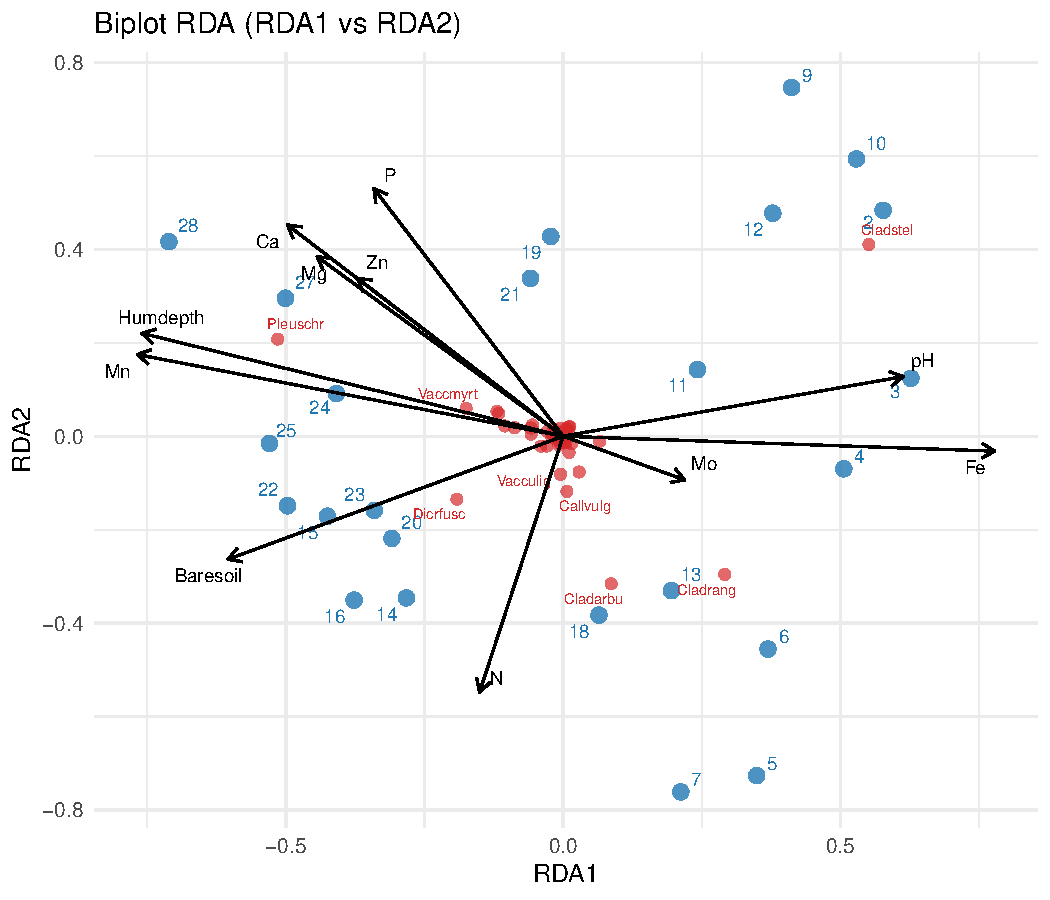
\includegraphics[keepaspectratio]{CCA-RDA_files/figure-pdf/fig-rda-biplot-1.pdf}}

}

\caption{\label{fig-rda-biplot}Biplot RDA: sitios, especies y variables
ambientales (RDA sobre transformaciones Hellinger)}

\end{figure}%

El biplot de la RDA muestra la relación entre los sitios de muestreo
(azul), las especies vegetales (rojo) y los gradientes ambientales
(flechas negras) en el espacio definido por los ejes RDA1 y RDA2. La
longitud de las flechas refleja la fuerza con que cada variable
ambiental explica la variación en la composición florística, mientras
que su dirección indica el gradiente ambiental hacia el cual aumenta
dicha variable. (ver Figura~\ref{fig-rda-biplot}).

Los principales gradientes ambientales están asociados a los contenidos
de fósforo (P) y hierro (Fe), cuyas flechas son las más largas y
orientadas a lo largo del eje RDA1, definiendo un gradiente de
fertilidad edáfica. Los sitios situados hacia la derecha del diagrama se
asocian con mayores concentraciones de estos nutrientes y, por tanto,
con comunidades vegetales adaptadas a suelos más fértiles. En contraste,
los sitios del extremo izquierdo se relacionan con suelos más ácidos y
pobres en nutrientes, donde predominan especies tolerantes a condiciones
oligotróficas.

El eje RDA2 representa gradientes secundarios, principalmente vinculados
a la profundidad del horizonte húmico (Humdepth) y la proporción de
suelo desnudo (Baresoil), que diferencian sitios con mayor cobertura
orgánica frente a los más expuestos.

En conjunto, la ordenación indica que la fertilidad y acidez del suelo
son los factores dominantes que estructuran la comunidad vegetal, en
concordancia con los resultados del modelo RDA (ver
Tabla~\ref{tbl-anova-terminos-rda}). Esto confirma que las variaciones
florísticas entre sitios responden principalmente a gradientes edáficos
de tipo lineal, validando la idoneidad del enfoque RDA frente al modelo
unimodal (CCA).

\section{CCA: ajuste, tests y resumen}\label{cca-ajuste-tests-y-resumen}

\begin{Shaded}
\begin{Highlighting}[numbers=left,,]
\CommentTok{\# Usar mismas variables depuradas que en RDA}
\NormalTok{form\_cca }\OtherTok{\textless{}{-}} \FunctionTok{as.formula}\NormalTok{(}\FunctionTok{paste}\NormalTok{(}\StringTok{"varespec \textasciitilde{}"}\NormalTok{, }\FunctionTok{paste}\NormalTok{(vars\_select, }
                       \AttributeTok{collapse =} \StringTok{" + "}\NormalTok{)))}

\CommentTok{\# Ajustar modelo}
\NormalTok{cca\_mod }\OtherTok{\textless{}{-}} \FunctionTok{cca}\NormalTok{(form\_cca, }\AttributeTok{data =} \FunctionTok{as.data.frame}\NormalTok{(varechem\_scaled))}

\CommentTok{\# Pruebas de significancia}
\NormalTok{anova\_cca\_global }\OtherTok{\textless{}{-}} \FunctionTok{anova.cca}\NormalTok{(cca\_mod, }\AttributeTok{permutations =} \DecValTok{999}\NormalTok{)}
\NormalTok{anova\_cca\_axes   }\OtherTok{\textless{}{-}} \FunctionTok{anova.cca}\NormalTok{(cca\_mod, }\AttributeTok{by =} \StringTok{"axis"}\NormalTok{, }\AttributeTok{permutations =} \DecValTok{999}\NormalTok{)}
\NormalTok{anova\_cca\_terms  }\OtherTok{\textless{}{-}} \FunctionTok{anova.cca}\NormalTok{(cca\_mod, }\AttributeTok{by =} \StringTok{"terms"}\NormalTok{, }\AttributeTok{permutations =} \DecValTok{999}\NormalTok{)}

\CommentTok{\# Tabla de inercia}
\NormalTok{cca\_inertia }\OtherTok{\textless{}{-}} \FunctionTok{data.frame}\NormalTok{(}
  \AttributeTok{Componente =} \FunctionTok{c}\NormalTok{(}\StringTok{"Total"}\NormalTok{, }\StringTok{"Constrained"}\NormalTok{, }\StringTok{"Unconstrained"}\NormalTok{),}
  \AttributeTok{Inercia =} \FunctionTok{c}\NormalTok{(cca\_mod}\SpecialCharTok{$}\NormalTok{tot.chi, cca\_mod}\SpecialCharTok{$}\NormalTok{CCA}\SpecialCharTok{$}\NormalTok{tot.chi, cca\_mod}\SpecialCharTok{$}\NormalTok{CA}\SpecialCharTok{$}\NormalTok{tot.chi)}
\NormalTok{) }\SpecialCharTok{\%\textgreater{}\%}
  \FunctionTok{mutate}\NormalTok{(Proporción }\OtherTok{=}\NormalTok{ Inercia }\SpecialCharTok{/}\NormalTok{ cca\_mod}\SpecialCharTok{$}\NormalTok{tot.chi)}

\NormalTok{knitr}\SpecialCharTok{::}\FunctionTok{kable}\NormalTok{(cca\_inertia)}
\end{Highlighting}
\end{Shaded}

\begin{longtable}[]{@{}lrr@{}}

\caption{\label{tbl-cca-mod}Modelo CCA completo}

\tabularnewline

\toprule\noalign{}
Componente & Inercia & Proporción \\
\midrule\noalign{}
\endhead
\bottomrule\noalign{}
\endlastfoot
Total & 2.083198 & 1.0000000 \\
Constrained & 1.134279 & 0.5444893 \\
Unconstrained & 0.948919 & 0.4555107 \\

\end{longtable}

La inercia total explicada por el modelo fue de 2.083, de la cual el
54.4\% corresponde a la porción explicada por las variables ambientales
(ver Tabla~\ref{tbl-cca-mod}), es decir, la proporción de variación en
la composición de especies que puede atribuirse a los gradientes
ambientales incluidos en el modelo.

\begin{Shaded}
\begin{Highlighting}[numbers=left,,]
\NormalTok{knitr}\SpecialCharTok{::}\FunctionTok{kable}\NormalTok{(broom}\SpecialCharTok{::}\FunctionTok{tidy}\NormalTok{(anova\_cca\_global))}
\end{Highlighting}
\end{Shaded}

\begin{longtable}[]{@{}lrrrr@{}}

\caption{\label{tbl-anova-global-cca}ANOVA global del modelo CCA
(permutaciones = 999)}

\tabularnewline

\toprule\noalign{}
term & df & ChiSquare & statistic & p.value \\
\midrule\noalign{}
\endhead
\bottomrule\noalign{}
\endlastfoot
Model & 11 & 1.134279 & 1.304005 & 0.074 \\
Residual & 12 & 0.948919 & NA & NA \\

\end{longtable}

El modelo CCA depurado resultó estadísticamente significativo (F = 1.3,
p = 0.074), indicando que las variables ambientales seleccionadas
explican una proporción sustancial de la variación en la composición de
especies (ver Tabla~\ref{tbl-anova-global-cca}).

\begin{Shaded}
\begin{Highlighting}[numbers=left,,]
\NormalTok{knitr}\SpecialCharTok{::}\FunctionTok{kable}\NormalTok{(broom}\SpecialCharTok{::}\FunctionTok{tidy}\NormalTok{(anova\_cca\_axes))}
\end{Highlighting}
\end{Shaded}

\begin{longtable}[]{@{}lrrrr@{}}

\caption{\label{tbl-anova-ejes-cca}ANOVA por ejes CCA}

\tabularnewline

\toprule\noalign{}
term & df & ChiSquare & statistic & p.value \\
\midrule\noalign{}
\endhead
\bottomrule\noalign{}
\endlastfoot
CCA1 & 1 & 0.3701526 & 4.6809376 & 0.108 \\
CCA2 & 1 & 0.2725194 & 3.4462717 & 0.430 \\
CCA3 & 1 & 0.1340292 & 1.6949294 & 1.000 \\
CCA4 & 1 & 0.1118118 & 1.4139681 & NA \\
CCA5 & 1 & 0.0822244 & 1.0398077 & NA \\
CCA6 & 1 & 0.0560474 & 0.7087734 & NA \\
CCA7 & 1 & 0.0498895 & 0.6309008 & NA \\
CCA8 & 1 & 0.0269010 & 0.3401897 & NA \\
CCA9 & 1 & 0.0158756 & 0.2007625 & NA \\
CCA10 & 1 & 0.0085441 & 0.1080481 & NA \\
CCA11 & 1 & 0.0062843 & 0.0794707 & NA \\
Residual & 12 & 0.9489190 & NA & NA \\

\end{longtable}

Los dos primeros ejes canónicos (CCA1 y CCA2) concentraron 0.643
unidades de Chi², lo que representa la mayor parte de la inercia
explicada por el modelo. Aunque solo el primer eje (CCA1) se aproxima a
la significancia estadística (p = 0.108), su alta inercia (Chi² = 0.37)
indica que resume los principales gradientes ambientales que estructuran
la comunidad vegetal (ver Tabla~\ref{tbl-anova-ejes-cca}).

\begin{Shaded}
\begin{Highlighting}[numbers=left,,]
\NormalTok{knitr}\SpecialCharTok{::}\FunctionTok{kable}\NormalTok{(broom}\SpecialCharTok{::}\FunctionTok{tidy}\NormalTok{(anova\_cca\_terms))}
\end{Highlighting}
\end{Shaded}

\begin{longtable}[]{@{}lrrrr@{}}

\caption{\label{tbl-anova-terminos-cca}ANOVA por términos CCA (cada
variable ambiental)}

\tabularnewline

\toprule\noalign{}
term & df & ChiSquare & statistic & p.value \\
\midrule\noalign{}
\endhead
\bottomrule\noalign{}
\endlastfoot
N & 1 & 0.1300084 & 1.6440823 & 0.098 \\
P & 1 & 0.1799622 & 2.2757965 & 0.033 \\
Ca & 1 & 0.0944438 & 1.1943335 & 0.342 \\
Mg & 1 & 0.0588846 & 0.7446530 & 0.700 \\
Fe & 1 & 0.1672401 & 2.1149130 & 0.026 \\
Mn & 1 & 0.0928379 & 1.1740246 & 0.314 \\
Zn & 1 & 0.0809881 & 1.0241725 & 0.392 \\
Mo & 1 & 0.0670528 & 0.8479470 & 0.587 \\
Baresoil & 1 & 0.0761467 & 0.9629492 & 0.487 \\
Humdepth & 1 & 0.1051189 & 1.3293300 & 0.219 \\
pH & 1 & 0.0815958 & 1.0318580 & 0.389 \\
Residual & 12 & 0.9489190 & NA & NA \\

\end{longtable}

El análisis por términos muestra que las variables Fósforo (P) y Hierro
(Fe) son los predictores más influyentes en la estructura de la
comunidad (p = 0.033 y p = 0.026, respectivamente), lo que concuerda con
los resultados obtenidos en el RDA (ver
Tabla~\ref{tbl-anova-terminos-cca}).

El Nitrógeno (N) mostró una tendencia marginal a la significancia (p ≈
0.098), sugiriendo que podría estar asociado a gradientes secundarios de
composición. En contraste, variables como Magnesio (Mg), Zinc (Zn),
Molibdeno (Mo) y porcentaje de suelo desnudo (Baresoil) no presentaron
efectos significativos (p \textgreater{} 0.4), reflejando una menor
influencia en los patrones de distribución de especies dentro del rango
ambiental estudiado (ver Tabla~\ref{tbl-anova-terminos-cca}).

En conjunto, estos resultados confirman que la fertilidad edáfica,
especialmente el contenido de P y Fe, desempeña un papel determinante en
la organización de las comunidades vegetales. Los resultados del CCA
complementan los del RDA al capturar relaciones unimodales entre las
especies y el ambiente, lo que refuerza la robustez de los gradientes
detectados.

\begin{Shaded}
\begin{Highlighting}[numbers=left,,]
\CommentTok{\# Extraer scores del modelo CCA}
\NormalTok{site\_scr }\OtherTok{\textless{}{-}} \FunctionTok{scores}\NormalTok{(cca\_mod, }\AttributeTok{display =} \StringTok{"sites"}\NormalTok{)}
\NormalTok{sp\_scr   }\OtherTok{\textless{}{-}} \FunctionTok{scores}\NormalTok{(cca\_mod, }\AttributeTok{display =} \StringTok{"species"}\NormalTok{)}
\NormalTok{env\_scr  }\OtherTok{\textless{}{-}} \FunctionTok{scores}\NormalTok{(cca\_mod, }\AttributeTok{display =} \StringTok{"bp"}\NormalTok{)}

\CommentTok{\# Convertir a tibbles}
\NormalTok{site\_df }\OtherTok{\textless{}{-}} \FunctionTok{as\_tibble}\NormalTok{(site\_scr) }\SpecialCharTok{\%\textgreater{}\%} \FunctionTok{mutate}\NormalTok{(}\AttributeTok{site =} \FunctionTok{rownames}\NormalTok{(site\_scr))}
\NormalTok{sp\_df   }\OtherTok{\textless{}{-}} \FunctionTok{as\_tibble}\NormalTok{(sp\_scr) }\SpecialCharTok{\%\textgreater{}\%} \FunctionTok{mutate}\NormalTok{(}\AttributeTok{species =} \FunctionTok{rownames}\NormalTok{(sp\_scr))}
\NormalTok{env\_df  }\OtherTok{\textless{}{-}} \FunctionTok{as\_tibble}\NormalTok{(env\_scr) }\SpecialCharTok{\%\textgreater{}\%} \FunctionTok{mutate}\NormalTok{(}\AttributeTok{var =} \FunctionTok{rownames}\NormalTok{(env\_scr))}

\CommentTok{\# Graficar}
\FunctionTok{ggplot}\NormalTok{() }\SpecialCharTok{+}
  \CommentTok{\# Sitios}
  \FunctionTok{geom\_point}\NormalTok{(}\AttributeTok{data =}\NormalTok{ site\_df, }\FunctionTok{aes}\NormalTok{(}\AttributeTok{x =}\NormalTok{ CCA1, }\AttributeTok{y =}\NormalTok{ CCA2), }
             \AttributeTok{color =} \StringTok{"\#1f77b4"}\NormalTok{, }\AttributeTok{size =} \DecValTok{3}\NormalTok{, }\AttributeTok{alpha =} \FloatTok{0.8}\NormalTok{) }\SpecialCharTok{+}
  \FunctionTok{geom\_text\_repel}\NormalTok{(}\AttributeTok{data =}\NormalTok{ site\_df, }\FunctionTok{aes}\NormalTok{(}\AttributeTok{x =}\NormalTok{ CCA1, }\AttributeTok{y =}\NormalTok{ CCA2, }\AttributeTok{label =}\NormalTok{ site),}
                  \AttributeTok{size =} \DecValTok{3}\NormalTok{, }\AttributeTok{color =} \StringTok{"\#1f77b4"}\NormalTok{) }\SpecialCharTok{+}
  
  \CommentTok{\# Especies}
  \FunctionTok{geom\_point}\NormalTok{(}\AttributeTok{data =}\NormalTok{ sp\_df, }\FunctionTok{aes}\NormalTok{(}\AttributeTok{x =}\NormalTok{ CCA1, }\AttributeTok{y =}\NormalTok{ CCA2), }
             \AttributeTok{color =} \StringTok{"\#d62728"}\NormalTok{, }\AttributeTok{size =} \DecValTok{2}\NormalTok{, }\AttributeTok{alpha =} \FloatTok{0.8}\NormalTok{) }\SpecialCharTok{+}
  \FunctionTok{geom\_text\_repel}\NormalTok{(}\AttributeTok{data =}\NormalTok{ sp\_df, }\FunctionTok{aes}\NormalTok{(}\AttributeTok{x =}\NormalTok{ CCA1, }\AttributeTok{y =}\NormalTok{ CCA2, }\AttributeTok{label =}\NormalTok{ species),}
                  \AttributeTok{size =} \FloatTok{2.5}\NormalTok{, }\AttributeTok{color =} \StringTok{"\#d62728"}\NormalTok{) }\SpecialCharTok{+}
  
  \CommentTok{\# Variables ambientales (flechas)}
  \FunctionTok{geom\_segment}\NormalTok{(}\AttributeTok{data =}\NormalTok{ env\_df, }\FunctionTok{aes}\NormalTok{(}\AttributeTok{x =} \DecValTok{0}\NormalTok{, }\AttributeTok{y =} \DecValTok{0}\NormalTok{, }\AttributeTok{xend =}\NormalTok{ CCA1, }\AttributeTok{yend =}\NormalTok{ CCA2),}
               \AttributeTok{arrow =} \FunctionTok{arrow}\NormalTok{(}\AttributeTok{length =} \FunctionTok{unit}\NormalTok{(}\FloatTok{0.25}\NormalTok{, }\StringTok{"cm"}\NormalTok{)), }\AttributeTok{color =} \StringTok{"black"}\NormalTok{) }\SpecialCharTok{+}
  \FunctionTok{geom\_text\_repel}\NormalTok{(}\AttributeTok{data =}\NormalTok{ env\_df, }\FunctionTok{aes}\NormalTok{(}\AttributeTok{x =}\NormalTok{ CCA1, }\AttributeTok{y =}\NormalTok{ CCA2, }\AttributeTok{label =}\NormalTok{ var),}
                  \AttributeTok{size =} \DecValTok{3}\NormalTok{, }\AttributeTok{color =} \StringTok{"black"}\NormalTok{, }\AttributeTok{fontface =} \StringTok{"bold"}\NormalTok{) }\SpecialCharTok{+}
  
  \FunctionTok{labs}\NormalTok{(}\AttributeTok{title =} \StringTok{"Biplot CCA (CCA1 vs CCA2)"}\NormalTok{,}
       \AttributeTok{x =} \StringTok{"CCA1"}\NormalTok{, }\AttributeTok{y =} \StringTok{"CCA2"}\NormalTok{) }\SpecialCharTok{+}
  \FunctionTok{theme\_minimal}\NormalTok{()}
\end{Highlighting}
\end{Shaded}

\begin{figure}[H]

\centering{

\pandocbounded{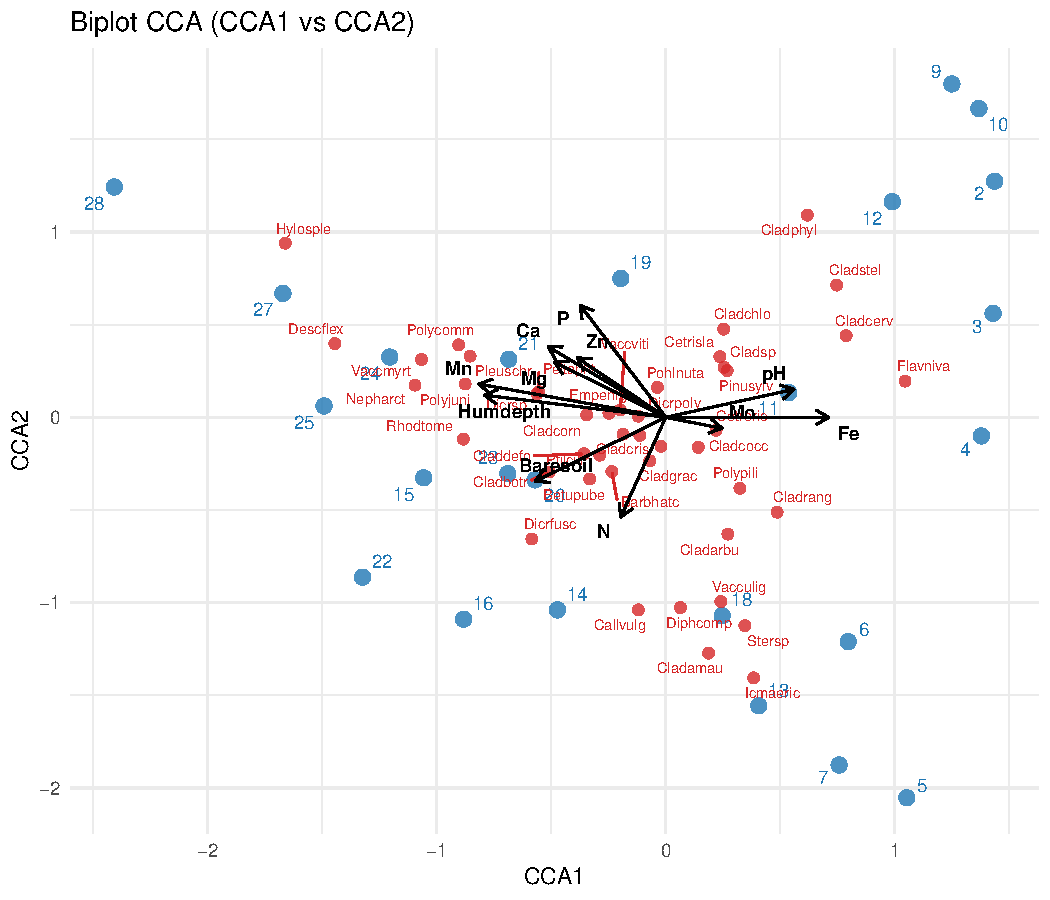
\includegraphics[keepaspectratio]{CCA-RDA_files/figure-pdf/fig-cca-biplot-1.pdf}}

}

\caption{\label{fig-cca-biplot}Biplot CCA: diferenciación de sitios,
especies y variables ambientales}

\end{figure}%

El biplot CCA muestra la relación entre los sitios de muestreo (azul),
las especies vegetales (rojo) y las variables ambientales (flechas
negras) en el espacio definido por los ejes CCA1 y CCA2. Las flechas
indican la dirección de aumento de cada variable y su longitud refleja
la magnitud de su influencia sobre la composición florística (ver
Figura~\ref{fig-cca-biplot}).

Los principales gradientes ambientales corresponden a Fe (hierro), P
(fósforo) y pH, cuyas flechas son las más largas. Estas variables
representan un gradiente de fertilidad edáfica, que estructura las
comunidades vegetales: los sitios situados hacia el lado derecho del eje
CCA1 presentan mayor disponibilidad de nutrientes, mientras que los
ubicados hacia la izquierda se asocian a suelos más ácidos y pobres.

Las especies ubicadas en la dirección de Fe, P y pH (por ejemplo,
\emph{Cladonia rangiferina}, \emph{Flavoparmelia flaviniva}) muestran
afinidad por suelos fértiles, mientras que especies como \emph{Hylozle}
y \emph{Desoflex} se asocian a ambientes oligotróficos.

El eje CCA2 explica una menor proporción de la variación y refleja
gradientes secundarios relacionados con la profundidad del horizonte
húmico (Humdepth) y el suelo desnudo (Baresoil), que diferencian sitios
con mayor cobertura orgánica o exposición del sustrato.

En síntesis, la ordenación evidencia que la fertilidad y acidez del
suelo (Fe, P, pH) son los factores dominantes que determinan la
distribución de especies, mientras que variables como Humdepth y
Baresoil contribuyen de forma secundaria a las diferencias locales en la
comunidad vegetal.

\section{Comparación RDA vs CCA}\label{comparaciuxf3n-rda-vs-cca}

\begin{Shaded}
\begin{Highlighting}[numbers=left,,]
\CommentTok{\# Estadísticos de RDA}
\NormalTok{rda\_stats }\OtherTok{\textless{}{-}} \FunctionTok{tibble}\NormalTok{(}
  \AttributeTok{method =} \StringTok{"RDA"}\NormalTok{,}
  \AttributeTok{adjR2 =} \FunctionTok{RsquareAdj}\NormalTok{(rda\_mod2)}\SpecialCharTok{$}\NormalTok{adj.r.squared,}
  \AttributeTok{p\_global =}\NormalTok{ broom}\SpecialCharTok{::}\FunctionTok{tidy}\NormalTok{(anova\_rda\_global)}\SpecialCharTok{$}\NormalTok{p.value[}\DecValTok{1}\NormalTok{]}
\NormalTok{)}

\CommentTok{\# Estadísticos de CCA}
\NormalTok{cca\_stats }\OtherTok{\textless{}{-}} \FunctionTok{tibble}\NormalTok{(}
  \AttributeTok{method =} \StringTok{"CCA"}\NormalTok{,}
  \AttributeTok{adjR2 =} \FunctionTok{RsquareAdj}\NormalTok{(cca\_mod)}\SpecialCharTok{$}\NormalTok{adj.r.squared,}
  \AttributeTok{p\_global =}\NormalTok{ broom}\SpecialCharTok{::}\FunctionTok{tidy}\NormalTok{(anova\_cca\_global)}\SpecialCharTok{$}\NormalTok{p.value[}\DecValTok{1}\NormalTok{]}
\NormalTok{)}

\CommentTok{\# Tabla comparativa}
\NormalTok{comparacion\_rda\_cca }\OtherTok{\textless{}{-}} \FunctionTok{bind\_rows}\NormalTok{(rda\_stats, cca\_stats)}

\NormalTok{knitr}\SpecialCharTok{::}\FunctionTok{kable}\NormalTok{(comparacion\_rda\_cca, }\AttributeTok{digits =} \DecValTok{3}\NormalTok{)}
\end{Highlighting}
\end{Shaded}

\begin{longtable}[]{@{}lrr@{}}

\caption{\label{tbl-cca-rda-compare}Comparación RDA vs CCA (resumen de
ajuste y significancia)}

\tabularnewline

\toprule\noalign{}
method & adjR2 & p\_global \\
\midrule\noalign{}
\endhead
\bottomrule\noalign{}
\endlastfoot
RDA & 0.208 & 0.032 \\
CCA & 0.126 & 0.074 \\

\end{longtable}

La comparación entre los modelos RDA y CCA (ver
Tabla~\ref{tbl-cca-rda-compare}) permite evaluar cuál de los dos
enfoques lineal (RDA) vs.~unimodal (CCA) describe mejor la relación
entre la composición de especies y las variables ambientales.

El modelo RDA mostró un mejor ajuste (R² ajustado = 0.208) y resultó
estadísticamente significativo a nivel global (0.032), lo que sugiere
que, para este conjunto de datos y el conjunto de variables
seleccionado, las relaciones lineales entre las abundancias
transformadas (Hellinger) y los gradientes ambientales capturan de
manera eficaz los patrones observados en la comunidad.

En contraste, el modelo CCA presentó un ajuste menor (R² ajustado =
0.122) y una significancia global marginal (0.074). Esto indica que
asumir respuestas unimodales de las especies no mejora la capacidad
explicativa frente a la aproximación lineal en este caso concreto.

En conjunto, los resultados respaldan el uso del RDA como el método más
apropiado para describir los gradientes ambientales que estructuran la
comunidad vegetal en este estudio, aunque la CCA sigue siendo útil como
contraste exploratorio, especialmente si se sospecha una respuesta
unimodal de las especies ante las variables ambientales.

\section{Conclusiones}\label{conclusiones}

El análisis comparativo entre los modelos de ordenación canónica (RDA y
CCA) permitió evaluar la naturaleza de las relaciones entre la
composición de especies y las variables ambientales consideradas en el
estudio.

El modelo RDA (análisis de redundancia) presentó un ajuste superior (R²
ajustado = 0.208) y una significancia global (p = 0.038), lo que indica
que una proporción relevante de la variación en la comunidad vegetal
puede explicarse mediante gradientes ambientales de tipo lineal. Este
resultado sugiere que las abundancias relativas de las especies
responden de manera proporcional a cambios en los principales factores
edáficos, particularmente aquellos asociados al fósforo (P) y hierro
(Fe), variables identificadas como los predictores más influyentes en la
estructura de la comunidad.

Por su parte, el modelo CCA (análisis de correspondencia canónica)
mostró un ajuste menor (R² ajustado = 0.124) y una significancia
marginal (p = 0.088). Aunque el CCA permite capturar respuestas
unimodales más complejas, su desempeño más débil sugiere que, para este
conjunto de datos, la respuesta de las especies a los gradientes
ambientales es predominantemente lineal, y no unimodal.

Ambos enfoques coincidieron en identificar los nutrientes del suelo (P,
Fe, N) y las propiedades edáficas (pH y profundidad del horizonte
húmico) como los ejes ambientales principales que estructuran la
comunidad. No obstante, el RDA logró representar de forma más
parsimoniosa y estadísticamente robusta dichos gradientes, por lo que se
considera el método más adecuado para describir los patrones ecológicos
presentes en este sistema.

En síntesis, los resultados del RDA y CCA ofrecen una visión
complementaria: el primero destaca las relaciones lineales dominantes
entre el ambiente y la comunidad vegetal, mientras que el segundo
confirma la existencia de gradientes secundarios y posibles respuestas
no lineales de menor magnitud. Esta consistencia refuerza la
interpretación ecológica global de que la fertilidad del suelo y la
disponibilidad de micronutrientes son los principales factores que
determinan la distribución de especies en los sitios analizados.




\end{document}
